
\documentclass[12pt]{article}
\raggedbottom
\usepackage[utf8]{inputenc}
\usepackage[T1]{fontenc}
\usepackage{newtxtext,newtxmath}        % Times New Roman

% Layout and spacing
\usepackage[margin=1in]{geometry}
\usepackage{setspace}
\usepackage{ragged2e}
\setlength{\RaggedRightParindent}{0.5in}
\usepackage{indentfirst}
\usepackage{etoolbox}
\usepackage{calc}

% Headings (JMF style)
\usepackage{titlesec}
\setcounter{secnumdepth}{0}
\titleformat{\section}{\normalfont\normalsize\centering\scshape}{}{0pt}{}
\titleformat{\subsection}{\normalfont\normalsize\centering\itshape}{}{0pt}{}
\titleformat{\subsubsection}{\normalfont\normalsize\raggedright\itshape}{}{0pt}{}
\titleformat{\paragraph}[runin]{\normalfont\normalsize\itshape}{}{0pt}{}[.]
\titlespacing*{\paragraph}{0.5in}{1ex}{0.5em}

% Figures and captions
\usepackage{graphicx}
\graphicspath{{./figures/}}
\usepackage{caption}
\usepackage{subcaption}
\captionsetup[table]{labelsep=period, justification=raggedright, singlelinecheck=false}
\captionsetup[figure]{labelsep=period, font=sc, justification=raggedright, singlelinecheck=false}

% Math
\usepackage{amsmath}
\usepackage{bm}
\usepackage{bbm}

% Tables
\usepackage{array}
\usepackage{booktabs}
\usepackage{makecell}
\usepackage{tabularx}
\usepackage{longtable}
\usepackage{threeparttable}
\usepackage{siunitx}
\sisetup{detect-all}
\usepackage[table]{xcolor}
\definecolor{Gray}{gray}{0.9}

% Floats and pages
\usepackage{float}
\floatstyle{plaintop}
\restylefloat{table}
\usepackage{floatrow}
\usepackage{placeins}
\usepackage{afterpage}
\usepackage{adjustbox}
\usepackage{pdflscape}
\usepackage{rotating}

% Misc
\usepackage{soul}
\usepackage{import}
\usepackage{url}
\newcommand\ddfrac[2]{\frac{\displaystyle #1}{\displaystyle #2}}

% Citations
\usepackage[round,sort]{natbib}
\setcitestyle{authoryear}

\usepackage[hidelinks]{hyperref}        % load last

\begin{document}
\doublespacing
\RaggedRight
\widowpenalty=10000
\clubpenalty=10000
\setlength{\parskip}{0ex}

% ---- Title page (page 1) ----
\thispagestyle{plain}
\begin{center}
Family Structure and the Well-Being of Pregnant Women in India, 2005--2021
\end{center}
\newpage

%%%%%%%%%%%%%%%%%%%%%%%%% ABSTRACT %%%%%%%%%%%%%%%%%%%%%%%%%


\section*{Abstract}

\noindent\textbf{Objective:} This study examines trends in pregnant women's residence in different household structures in India from 2005 to 2021 and how their autonomy and healthcare use differ by household types over time. 

\medskip
\noindent\textbf{Background:}Research on young women in India that studies the 1990s to the early 2000s documents a shift away from patrilocal extended family residence towards nuclear households, and suggests trade-offs between women’s autonomy and access to resources across household types.

\medskip
\noindent\textbf{Method:} Using three rounds of nationally representative data from India, the National Family and Health Survey data (2005--06, 2015--16 and 2019--21) this study analyses currently pregnant women and compares between autonomy and healthcare use across household types and assess the change in these relationships over time.  

\medskip
\noindent\textbf{Results:} Between 2005 and 2021, pregnant women increasingly lived in patrilocal extended households. Those in extended households had less decision making power but greater healthcare use than those in nuclear households, but this gap has also narrowed over time.

\medskip
\noindent\textbf{Conclusion:} Contrary to the expectation of linking modernization with nuclear families, pregnancy in India increasingly occurs within extended patrilocal households. But these results may not have the consequences implied by the prior literature on family structure.

\medskip
\noindent\textbf{Implications:} These results speaks to the growing literature on demographic change in India where the trend towards pregnancy and parenthood occurring in extended families may continue as grandparents live longer and successive generations have smaller families and research should reassess what it meand for women's well being. 


 
\vspace*{12pt}

\setlength{\parskip}{0ex}

\pagestyle{fancy}
\setcounter{footnote}{\autorzahl}
\newpage

%%%%%%%%%%%%%%%%%%%%%%%%%%%% MAIN TEXT %%%%%%%%%%%%%%%%%%%%%%%%%%%

% \newpage % remove if abstract continues to second page
\section*{Introduction}\label{sec:Introduction} % remember to change the label if the authors use a different one

India, home to one in six of the world’s births, provides an important context to examine how family relationships and household structure shape maternal health and well being. A growing literature links women's marital and family context to health through mechanisms such as chronic stress and cumulative disadvantage associated with early marriage \citep{vikram2021early}. Although pregnancy occurs almost exclusively within the context of marriage \citep{banerji2021does}, there is substantial variation in the types of families in which pregnant women reside. Women may live in nuclear households, consisting of only the couple and their children, or they may live in patrilocal extended family households in which a woman resides with her husband’s parents, siblings, and other relatives.  They may also live with their natal kin.

Patrilocal extended family residence has historically been the normative family structure in India.  Explanations for the societal emphasis on this family structure include that sons, rather than daughters, can expect to to inherit land and property, and that sons are more likely to be seen as responsible for providing old-age support for their parents \citep{dyson1983kinship, pande2007explaining, allendorf2020another, pandian2022rise}. Research on the demographic consequences of modernization and the status of women in India has noticed that a large and modestly increasing fraction of households in India were nuclear during the period from 1983 to 2009 \citep{breton2021modernisation}.  Similarly, \cite{allendorf2013going} observed that between 1991 and 2005, women of childbearing age were 8 percentage points more likely to live in nuclear families, rather than patrilocal extended families.

This study focuses specifically on pregnant women. We find that from the 1990s to early 2000s, the proportion of pregnant women living it patrilocal extended households was fairly stable, but that there was an increase between 2005 and 2021.  Figure [INSERT NEW FIGURE] illustrates this trend by showing the proportion of pregnant women residing in natal, patrilocal extended and nuclear family households at the time of each of India's five National Family Health Surveys.  Table \ref{tab:patrilocal_subgroups} uses data from the three most recent rounds of India's National Family Health Surveys to show that pregnant women are 9 percentage points more likely to be living in a patrilocal extended household in 2021 than they were in 2005.  Perhaps surprisingly, considering \cite{dyson1983kinship}'s observation that, at the time of the paper's publication, nuclear households were more common in the South than the North, Table \ref{tab:patrilocal_subgroups} also shows that nearly 3 in 4 pregnant women in the South now resides with her in-laws.  With the exception of the northeastern states which account for less than 5\% of the Indian population, rates of patrilocal extended family residence among pregnant women are over 60\% in all regions.  Table \ref{tab:patrilocal_subgroups} also shows that patrilocal extended family residence is not restricted to a particular social or age group, though it is least common among Muslims and older women.

% \begin{table}[H]
% \caption{: Proportion of pregnant women in patrilocal extended households is increasing among nearly all subgroups}
% \label{tab:patrilocal_subgroups}
% \vspace{-4pt}

% \begin{scriptsize}
% \setlength{\tabcolsep}{6pt}
% \renewcommand{\arraystretch}{1.2}

% \makebox[\linewidth][c]{%
%     \begin{tabular}{lcccc}
\toprule
 & \multicolumn{1}{c}{2005--2006} & \multicolumn{1}{c}{2015--2016} & \multicolumn{1}{c}{2019--2021} & \multicolumn{1}{c}{\shortstack{p-value\\2005--2006 vs.\\2019--2021}} \\
\midrule
\textbf{All currently pregnant women}&0.61&0.69&0.70&0.00\\
&&&&\\
\textbf{Social group}&&&&\\
\hspace*{2em}Adivasi&0.53&0.66&0.70&0.00\\
\hspace*{2em}Dalit&0.55&0.64&0.70&0.00\\
\hspace*{2em}OBC&0.63&0.73&0.75&0.00\\
\hspace*{2em}Forward caste&0.71&0.80&0.70&0.03\\
\hspace*{2em}Muslim&0.55&0.59&0.58&0.03\\
\hspace*{2em}Sikh/Jain/Christian&0.78&0.74&0.81&0.53\\
&&&&\\
\textbf{Region$^1$}&&&&\\
\hspace*{2em}Uttar Pradesh and Bihar&0.60&0.68&0.67&0.00\\
\hspace*{2em}Central&0.57&0.70&0.71&0.00\\
\hspace*{2em}East&0.63&0.64&0.62&0.48\\
\hspace*{2em}West&0.65&0.76&0.82&0.00\\
\hspace*{2em}North&0.65&0.77&0.79&0.00\\
\hspace*{2em}South&0.58&0.67&0.72&0.00\\
\hspace*{2em}Northeast&0.51&0.56&0.54&0.01\\
&&&&\\
\textbf{Age}&&&&\\
\hspace*{2em}15--19&0.76&0.86&0.83&0.00\\
\hspace*{2em}20--24&0.67&0.75&0.78&0.00\\
\hspace*{2em}25--29&0.52&0.66&0.64&0.00\\
\hspace*{2em}30--34&0.39&0.51&0.56&0.00\\
\hspace*{2em}35--39&0.27&0.38&0.34&0.01\\
\hspace*{2em}40--44&0.28&0.49&0.35&0.95\\
\hspace*{2em}45--49&0.09&0.13&0.00&0.82\\
&&&&\\
\textbf{Parity (live births)}&&&&\\
\hspace*{2em}0&0.78&0.83&0.84&0.00\\
\hspace*{2em}1&0.65&0.71&0.69&0.00\\
\hspace*{2em}2&0.55&0.55&0.60&0.07\\
\hspace*{2em}3+&0.38&0.43&0.40&0.78\\
&&&&\\
\textbf{N (currently pregnant women)}&4,390&3,998&3,037&\\
\bottomrule
\end{tabular}
%
% }

% \end{scriptsize}

% \vspace{1ex}
% \small\scriptsize{\textsf{\textit{Note}: Data are from NFHS rounds 3 (2005--2006), 4 (2015--2016), and 5 (2019--2021).}} 
% \small\scriptsize{\textsf{The sample is restricted to ever-married women in either nuclear or patrilocal extended household structures, and women who report being three or more months pregnant when surveyed.}}
% \newline
% \small\scriptsize{\textsf{P-values are from weighted linear probability models regressing patrilocal extended household residence on an indicator for 2019--2021, in which being from the 2005--2006 round is the omitted category. Samples are restricted to the relevant subgroup. Standard errors are clustered at the primary sampling unit level.}}
% \newline
% \small\scriptsize{\textsf{$^1$ Central includes Madhya Pradesh and Chhattisgarh. East includes West Bengal, Jharkhand, and Odisha. West includes Gujarat, Maharashtra, and Goa. North includes Jammu and Kashmir, Himachal Pradesh, Punjab, Uttarakhand, Haryana, and Rajasthan. South includes Andhra Pradesh, Karnataka, Kerala, Tamil Nadu, and Telangana. Northeast includes Arunachal Pradesh, Assam, Manipur, Meghalaya, Mizoram, Nagaland< Sikkim and Tripura. Uttar Pradesh and Bihar are listed separately because they have a large burden of poor maternal health outcomes.}}
% \end{table}

\vspace{1.5\baselineskip}


\begin{scriptsize}
\setlength{\tabcolsep}{6pt}
\renewcommand{\arraystretch}{1.2}

\captionof{table}{ Proportion of pregnant women in patrilocal extended households is increasing among nearly all subgroups}
\label{tab:patrilocal_subgroups}

\vspace{-4pt}

\begingroup

% Center the longtable
\setlength\LTleft{\fill}
\setlength\LTright{\fill}

% Temporarily interpret the Stata-generated tabular as longtable
\let\tabular\longtable
\let\endtabular\endlongtable

\begin{tabular}{lcccc}
\toprule
 & \multicolumn{1}{c}{2005--2006} & \multicolumn{1}{c}{2015--2016} & \multicolumn{1}{c}{2019--2021} & \multicolumn{1}{c}{\shortstack{p-value\\2005--2006 vs.\\2019--2021}} \\
\midrule
\textbf{All currently pregnant women}&0.61&0.69&0.70&0.00\\
&&&&\\
\textbf{Social group}&&&&\\
\hspace*{2em}Adivasi&0.53&0.66&0.70&0.00\\
\hspace*{2em}Dalit&0.55&0.64&0.70&0.00\\
\hspace*{2em}OBC&0.63&0.73&0.75&0.00\\
\hspace*{2em}Forward caste&0.71&0.80&0.70&0.03\\
\hspace*{2em}Muslim&0.55&0.59&0.58&0.03\\
\hspace*{2em}Sikh/Jain/Christian&0.78&0.74&0.81&0.53\\
&&&&\\
\textbf{Region$^1$}&&&&\\
\hspace*{2em}Uttar Pradesh and Bihar&0.60&0.68&0.67&0.00\\
\hspace*{2em}Central&0.57&0.70&0.71&0.00\\
\hspace*{2em}East&0.63&0.64&0.62&0.48\\
\hspace*{2em}West&0.65&0.76&0.82&0.00\\
\hspace*{2em}North&0.65&0.77&0.79&0.00\\
\hspace*{2em}South&0.58&0.67&0.72&0.00\\
\hspace*{2em}Northeast&0.51&0.56&0.54&0.01\\
&&&&\\
\textbf{Age}&&&&\\
\hspace*{2em}15--19&0.76&0.86&0.83&0.00\\
\hspace*{2em}20--24&0.67&0.75&0.78&0.00\\
\hspace*{2em}25--29&0.52&0.66&0.64&0.00\\
\hspace*{2em}30--34&0.39&0.51&0.56&0.00\\
\hspace*{2em}35--39&0.27&0.38&0.34&0.01\\
\hspace*{2em}40--44&0.28&0.49&0.35&0.95\\
\hspace*{2em}45--49&0.09&0.13&0.00&0.82\\
&&&&\\
\textbf{Parity (live births)}&&&&\\
\hspace*{2em}0&0.78&0.83&0.84&0.00\\
\hspace*{2em}1&0.65&0.71&0.69&0.00\\
\hspace*{2em}2&0.55&0.55&0.60&0.07\\
\hspace*{2em}3+&0.38&0.43&0.40&0.78\\
&&&&\\
\textbf{N (currently pregnant women)}&4,390&3,998&3,037&\\
\bottomrule
\end{tabular}

\addtocounter{table}{-1}

\endgroup

\vspace{1ex}

\textsf{\textit{Note}: Data are from NFHS rounds 3 (2005--2006),
4 (2015--2016), and 5 (2019--2021).}

\textsf{The sample is restricted to ever-married women in either nuclear
or patrilocal extended household structures, and women who report being
three or more months pregnant when surveyed.}

\textsf{P-values are from weighted linear probability models regressing
patrilocal extended household residence on an indicator for 2019--2021,
in which being from the 2005--2006 round is the omitted category.
Samples are restricted to the relevant subgroup. Standard errors are
clustered at the primary sampling unit level.}

\textsf{$^1$ Central includes Madhya Pradesh and Chhattisgarh. East
includes West Bengal, Jharkhand, and Odisha. West includes Gujarat,
Maharashtra, and Goa. North includes Jammu and Kashmir, Himachal Pradesh,
Punjab, Uttarakhand, Haryana, and Rajasthan. South includes Andhra Pradesh,
Karnataka, Kerala, Tamil Nadu, and Telangana. Northeast includes Arunachal
Pradesh, Assam, Manipur, Meghalaya, Mizoram, Nagaland, Sikkim, and Tripura.
Uttar Pradesh and Bihar are listed separately because they have a large
burden of poor maternal health outcomes.}

\end{scriptsize}

\vspace{1.5\baselineskip}


What may be the consequences of this shift in family structure for the well being of pregnant women? Research on co-residence with in-laws during pregnancy in South Asia has tended to find that co-residence with in-laws is associated with adverse pregnancy experiences such as domestic violence, abuse, and unsupportive household environments \citep{silverman2016maternal,kazi2006social,raj2011abuse}.  More broadly, the prior literature describes how family structures shape the social context in which women live, as well as their social status. Newly married women in patrilocal extended households occupy the lowest position in both gender and generational hierarchies. Daughters-in-law in patrilocal extended households are valued for childbearing and labor, but are disadvantaged by limitations on their labor force participation and by inheritance systems that privilege men \citep{afridi2018fewer, mookerjee2019gender, reed2020labor, chatterjee2022women}.  

\cite{khalil2019patrilocal} find that women in patrilocal extended families have less decision-making power than those in nuclear households, and that these differences are unlikely to be due to selection into household type. Indeed, patrilocal households have more wealth than nuclear ones, and women who live with their in-laws are, on average, more educated than women living in nuclear households, as are their husbands.  Each of these variables -- wealth and education -- is independently associated with greater decision-making power among women.

This paper builds on prior empirical research by \cite{allendorf2013going}, who uses Indian data from 1992, 1999, and 2005 and looks at trends for women of child-bearing age (rather than pregnant women \emph{per se}).  Our findings cohere with  \cite{allendorf2013going}'s characterizations of nuclear and patrilocal extended households, with important updates.  In all three of the survey rounds that we analyze -- from 2005, 2015, and 2021 -- pregnant women in patrilocal extended households have less decision-making power relative to pregnant women in nuclear households, but are more likely to use maternal healthcare. Consistent with the periods that \cite{allendorf2013going} and \cite{khalil2019patrilocal} studied, we find that patrilocal extended households are wealthier than nuclear families, and that wealth mediates the relationship between maternal healthcare use and household type. 

We advance the literature by showing that these relationships have changed in important ways in the the past two decades.  Differences by household type in both women's decision-making and maternal healthcare use have narrowed significantly, which is consistent with rapid improvement in the accessibility of maternal healthcare during this period \citep{gandhi2022predictors, rai2022use}, as well as with important increases in women's decision-making power across household types.  

To summarize this paper's contributions to the literature: it documents a new trend in the family context in which pregnancies take place, and it shows weakening of the relationships between family structure and outcomes that matter for pregnant women's well being over time.  Finally, it provides a counterexample to the literature which finds or assumes that women's decision-making power determines maternal healthcare use \citep{majumder2024does,mistry2009women}.  In this context, maternal healthcare use is shaped by other factors, such as economic resources.  

Although it is beyond the scope of this paper to assess the reasons why pregnancy and parenthood in India increasingly take place in the context of an extended family, the likely explanations -- that in-laws live longer, that women complete childbearing at younger ages, and that men have fewer brothers to look after aging parents -- are all demographic patterns that are likely to continue in the future.  This perhaps increases the value of documenting trends in pregnant women's well being by family structure during the period we study.

\subsection*{The well being of pregnant women in patrilocal extended and nuclear households}

Ethnographic and sociological work documents that young daughters-in-law in extended patrilocal households are expected to demonstrate deference to senior family members, take on a disproportionate share of domestic labor, and face restrictions on mobility and decision-making \citep{mandelbaum1988women, jeffery1989labour, gupta1999lifeboat}.  Parents-in-law, and especially mothers-in-law, exercise control over the daily lives of their daughters-in-law \citep{desai2005women, bloom2001dimensions}. 

The impact on maternal well being of a woman's position as daughter-in-law can occur through many pathways. Other family members may control spending, or not invest adequately in maternal health \citep{ganle2015intra,raj2011abuse}. Pregnant daughters-in-law may have limited ability to take rest or travel for healthcare due to their burden of housework. Daughters-in-law may not get enough to eat when they are pregnant. Mothers facing discrimination and stress may develop mental health problems that affect maternal health. \cite{coffey2022mothers} find that lower women’s status in patrilocal extended households can be linked to lower survival rates and worse health outcomes for children, likely due to worse nutrition among low-status mothers.

However, patrilocal extended family residence may also offer advantages for pregnant women, shaping their well-being through multiple mechanisms.  The presence of other adult family members can provide support in the form of shared domestic labor and childcare, which may free up women’s time for other activities \citep{khanna2024role}. Co-residence with extended family members may reduce the likelihood of spousal violence \citep{khanna2024role, khalil2019patrilocal, allendorf2013going}. Additionally, mothers-in-law and other female household members may be a valuable resource during pregnancy in ensuring that women are getting the care they need \citep{varghese2019coresidence}.  Patrilocal extended households may be characterized by pooled economic resources, intergenerational support, and shared domestic labor \citep{wadley1988karimpur}.  

Nuclear households, in contrast, may provide greater scope for spousal communication and individual autonomy, but may lack the economic and caregiving support available in extended families. Married women in nuclear households are less likely to face the same pressure from their in-laws. The absence of a senior kin may increase women’s participation in household decision-making \citep{simkhada2010role,char2010influence}. For example, \cite{mookerjee2019gender} finds that shifts from patrilocal extended to nuclear households increase women’s mobility and participation in decision-making by reducing the control exerted by extended family members. Further, when husbands in nuclear households migrate for work, women become the head of the household, assuming primary responsibility for  household management, further enhancing her decision-making authority \citep{desai2008negotiated}. 

\section*{Data and methods}\label{sec:data_and_methods} % remember to change the label if the authors use a different one

\subsection*{Data} \label{sec:data}

We use data from India’s National Family Health Survey (NFHS) rounds 3 (2005–2006), 4 (2015–2016), and 5 (2019–2021). The NFHS is India’s Demographic and Health Survey, a nationally representative cross-sectional survey of households and women aged 15–49. These data are publicly available from \url{https://www.dhsprogram.com}.

The sample for our primary analyses on trends in household structure and their relationship with autonomy outcomes are women who are ever married, currently pregnant, and living in either a nuclear or patrilocal household structure. Appendix Table B-1 shows that women who report being one or two months pregnant differ systematically from those reporting three or more months of pregnancy. In particular, early pregnancy is more likely to be recognized or reported among more educated and wealthier women. We therefore exclude women reporting one or two months of pregnancy from the analysis. We exclude women living in natal households (about 15\% of the sample), as this living arrangement represents a substantively different social context from both patrilocal and nuclear households. For example, \cite{dyson1983kinship} explain that closer ties to the natal families indicate higher autonomy for women.The prevalence of visiting to one's natal residence among pregnant women is stable across survey rounds and has further reduced over the survey rounds, as seen in Appendix Figure C-1.  Excluding this group does not affect the interpretation of trends. For analyses of maternal healthcare use, instead of focusing on pregnant women, we restrict the sample to ever married women who gave birth in the 3--12 months before the survey.

\subsection*{Variables}

\subsubsection*{Household structure} \label{sec:def_hhstruc}
We construct the household structure variable using information on the people residing in the same household as the pregnant woman. We define nuclear households as ones where the woman and her husband are the only two adult members in the household. Patrilocal extended households are defined as the ones where the woman lives with her husband’s adult kin, such as her parent-in-law or adult sibling-in-law. Natal households are those in which the pregnant woman is the daughter or the sister of the household head and none of her husband’s adult kin are present. 

\subsubsection*{Decision-making and healthcare use} \label{sec:outcomes}
To understand women's autonomy during pregnancy, we construct outcomes based on answers to two questions: ``Who usually makes decisions about health care for yourself?'' and ``Who usually makes decisions about visits to your family or relatives?'' We dichotomize these measures by coding women who report that their husband or someone else makes the decision on their behalf as having ‘no say,’ and those who report deciding jointly with their husband or being the only decision maker as ‘some say.’

To measure maternal healthcare use among recently postpartum women, we examine two indicators: birth in a health facility (as opposed to at home) and having four or more prenatal visits. The four visit threshold follows the World Health Organization (WHO) and Government of India’s National Health Mission guidelines from 2016.In 2016 WHO and NRHM increased the recommended minimum number of visits to 8.  We use 4 because the median pregnant woman in our data was pregnant in 2015.

\subsubsection*{Sociodemographic variables}  

We define social groups by combining caste and religion, as recommended by the India Human Development Survey \citep{desai2008india}. Women are classified as Adivasi or Dalit if they report belonging to a Scheduled Tribe or Scheduled Caste, respectively. Muslim women who are not Scheduled Tribe (ST) or Scheduled Caste (SC) are classified as Muslim. Hindu or Sikh women belonging to Other Backward Classes are classified as OBC. Hindu women who are not SC, ST, or OBC are classified as Forward caste. Women who do not fall into these categories (e.g., Christian, Jain, Sikh outside OBC, or no religion) are excluded. 

Uttar Pradesh and Bihar are separated as focus states within regions since they have the highest neonatal mortality in the country \citep{coffey2025excess}. 

\subsubsection*{Household wealth} \label{sec:wealthcontrols}

To capture differences in wealth across household types, we construct a categorical wealth measure based on the full interaction of 8 asset ownership indicators, which has 784 categories. Households are grouped into mutually exclusive categories defined by all combinations of ownership of finished floors, electricity, a radio, a television, a refrigerator, a bicycle, a car, and a latrine or toilet, and these categories are included as fixed effects.

\subsection*{Analysis}
\subsubsection*{OLS linear probability models of autonomy and healthcare use outcomes on family structure}

We estimate ordinary least squares (OLS) linear probability models to examine the association between household structure and the four binary outcomes: (1) reporting ``no say'' in decisions about the respondent's own healthcare, (2) reporting ``no say'' in decisions about visits to family or relatives, (3) having an institutional delivery (birth in a health facility), and (4) receiving at least four prenatal visits. We use these models because the coefficients can be directly interpreted as percentage point differences, which facilitates comparison across outcomes and survey rounds. In our data, the outcomes are not extremely rare, so linear models provide a reasonable approximation.  Our baseline specification controls for state of residence because both health care use and women's decision making vary by state.
We use relatively simple models without a large number of control variables because the purpose of this analysis is not to identify a causal effect of household structure on the outcomes.  We interpret the existing literature to have established the links between these outcomes and household structure.  We are most interested in understanding whether the relationships still exist in updated data, and whether the magnitudes of differences by family structure are changing over time.

For woman $i$ in state $s$, we estimate:

\begin{equation} \label{eq:nocontrols}
Y_{is} = \beta_0 + \beta_1 \text{Patrilocal}_{is} + \mu_s + \epsilon_{is},
\end{equation}

where $i$ indexes women and $s$ indexes states. $Y_{is}$ denotes the outcomes described above, $\text{Patrilocal}_{is}$ is an indicator for residing in a patrilocal extended household (with nuclear households as the reference category), $\mu_s$ are state fixed effects, and $\epsilon_{is}$ is an error term. We estimate this equation separately for each NFHS round to examine how the relationships between household structure and the outcomes change over time.

Because the prior literature established household economic status as a mediator for these relationships, we estimate an additional specification that includes $\lambda_{is}$, the wealth group fixed effects described above:

\begin{equation} \label{eq:controls}
Y_{is} = \beta_0 + \beta_1 \text{Patrilocal}_{is} + \lambda_{is} + \mu_s + \epsilon_{is}.
\end{equation}

In all models, we report standard errors clustered at the primary sampling unit level to account for within-cluster correlation of outcomes.All models account for the NFHS complex survey design using sampling weights and stratification.

\subsubsection*{Changes in patrilocal–nuclear differences across survey rounds}

To examine how differences between patrilocal extended and nuclear households evolve over time, we estimate models that allow the association between household structure and outcomes to vary across survey rounds. Specifically, for comparisons between 2005--2006 and 2015--2016, as well as 2015--2016 and 2019--2021, we estimate the following OLS linear probability models:

\begin{equation} \label{eq:tworounds}
Y_{is} = \alpha + \beta \,\text{Patrilocal}_i + \gamma \,\text{LaterRound}_t
+ \delta \,(\text{Patrilocal}_i \times \text{LaterRound}_t)
+ \lambda_{g(i)} + \mu_s + \varepsilon_{is},
\end{equation}


where $Y_{is}$ are the outcomes described above, $\text{LaterRound}_t$ is an indicator for the later survey round in the comparison. The coefficient of interest $\delta$ captures the change in the patrilocal-nuclear gap between the two survey rounds. As in the main specification, $\lambda_{g(i)}$ denotes wealth-group fixed effects, and $\mu_s$ denotes state fixed effects. This approach allows us to directly test whether the patrilocal–nuclear gap changes across survey rounds, and to assess the statistical significance of these changes.

We also estimate a pooled specification including all three survey rounds to assess changes in the patrilocal-nuclear gap across rounds while using the full sample. The equation is:

\begin{equation} \label{eq:stacked}
\begin{aligned}
Y_{is} = \alpha 
&+ \beta \,\text{Patrilocal}_i
+ \gamma_4 \,\text{NFHS-4}_t
+ \gamma_5 \,\text{NFHS-5}_t \\
&+ \delta_4 \,(\text{Patrilocal}_i \times \text{NFHS-4}_t)
+ \delta_5 \,(\text{Patrilocal}_i \times \text{NFHS-5}_t) \\
&+ \lambda_{g(i)} + \mu_s + \varepsilon_{is}.
\end{aligned}
\end{equation}

2005--2006 is the omitted category; NFHS-4 refers to 2015--2016, and NFHS-5 refers to 2019--2021. $\lambda_{g(i)}$ denotes wealth-group fixed effects, and $\mu_s$ denotes state fixed effects. The reported coefficients $\delta_4$ and $\delta_5$ measure changes in the patrilocal-nuclear gap relative to the gap in 2005--2006.





\section*{Results}
% \subsection*{Increasing patrilocal residence among pregnant women}

% Table \ref{tab:patrilocal_subgroups} shows that the share of pregnant women living in patrilocal extended households increased from 61\% in 2005–2006 to 70\% in 2019–2021. This increase is observed across all social groups, with particularly large increases among Adivasi women (17 percentage points), and a smaller increase for Muslim women at 3 percentage points.

% Patrilocal residence increased in all regions except the East. In 2019--2021, patrilocal residence is highest in the North and West (79 and 82 percent, respectively), but even areas with comparatively lower baseline levels of patrilocal residence such as Northeast and South showed a noticeable increase in patrilocal residence.  

% Patrilocal residence varies sharply by age and parity. Younger women are substantially more likely to live in patrilocal extended households than older women: in 2019–2021, 83\% of pregnant women aged 15–19 reside in patrilocal households, compared to less than 35\% among women aged 40–44. Similarly, women with lower parity are more likely to reside in patrilocal households. These patterns are consistent with patrilocal extended household residence being most common in the early stages of marriage and childbearing. While the likelihood of living in extended families declines with age and parity, increases over time are observed across most age and parity groups. 


\subsection*{Extended family residence predicts maternal healthcare use and autonomy}

Table \ref{tab:sumstats} presents summary statistics for autonomy, maternal healthcare use, and wealth outcomes by household structure. Among currently pregnant women, there are large and persistent differences in decision-making power by household type. In 2005–2006, 51\% of women in patrilocal extended households report having no say in their own healthcare, compared to 32\% of women in nuclear households. By 2019–2021, these shares decline to 25\% and 18\% respectively. While autonomy improves substantially over time for both groups, the gap between household types narrows considerably, from 19 percentage points in 2005–2006 to 7 percentage points in 2019–2021. A similar pattern is observed for women’s ability to visit family and friends, where differences of comparable magnitude persist across all survey rounds.

In contrast, maternal healthcare use is higher for women in patrilocal extended households. Among women who gave birth in the 3–12 months preceding the survey, 45\% of women in patrilocal households delivered in a health facility in 2005–2006, compared to 34\% in nuclear households. By 2019–2021, although institutional delivery rates increased dramatically for both groups, to 93\% in patrilocal households and 86\% in nuclear households, the advantage for patrilocal households remained. A similar pattern is observed for prenatal care: the share of women receiving four or more visits rises from 40 to 61\% in patrilocal households and from 31 to 53\% in nuclear households over the same period. Thus, while overall access to maternal healthcare improved substantially, differences by household structure persist.

As in the prior literature, household wealth mediates maternal health care use differences across households structures. Across all survey rounds and for nearly all indicators, women in patrilocal extended households are more likely to live in households with higher asset ownership and better housing conditions. For example, in 2019–2021, 59\% of pregnant women in patrilocal households live in homes with finished floors compared to 51\% in nuclear households, and 83\% in patrilocal extended household have access to a toilet or latrine compared to 78\% in nuclear households. Ownership of consumer durables such as televisions and refrigerators is also substantially higher in patrilocal households.


\begin{table}[H]
\caption{: Pregnant women in patrilocal extended households are advantaged in wealth and maternal healthcare use, but disadvantaged in autonomy outcomes}
\label{tab:sumstats}
\vspace{-4pt}

\begin{scriptsize}
\setlength{\tabcolsep}{7pt}
\renewcommand{\arraystretch}{1.15}

\makebox[\linewidth][c]{%
\begin{tabular}{lccccccccc}
\toprule
 & \multicolumn{3}{c}{2005--2006} & \multicolumn{3}{c}{2015--2016} & \multicolumn{3}{c}{2019--2021} \\
\cmidrule(lr){2-4} \cmidrule(lr){5-7} \cmidrule(lr){8-10}
 & Nuclear & \shortstack{Patrilocal\\Extended} & Sig. & Nuclear & \shortstack{Patrilocal\\Extended} & Sig. & Nuclear & \shortstack{Patrilocal\\Extended} & Sig. \\
\midrule
\textbf{\shortstack[l]{Autonomy measures\\(pregnant sample)}}&&&&&&&&&\\
No say in own healthcare&0.32&0.52&***&0.26&0.32&***&0.18&0.25&***\\
No say in visits to family/friends&0.32&0.56&***&0.25&0.35&***&0.17&0.25&***\\
&&&&&&&&&\\
\textbf{\shortstack[l]{Healthcare measures\\(recent birth sample)}}&&&&&&&&&\\
Birth in a health facility&0.34&0.45&***&0.77&0.86&***&0.86&0.93&***\\
4+ prenatal visits&0.31&0.40&***&0.45&0.55&***&0.53&0.61&***\\
&&&&&&&&&\\
\textbf{\shortstack[l]{Wealth measures\\(pregnant sample)}}&&&&&&&&&\\
Finished floor&0.32&0.43&***&0.46&0.54&***&0.51&0.59&***\\
Electricity&0.60&0.70&***&0.80&0.88&***&0.94&0.97&***\\
Owns radio&0.26&0.38&***&0.06&0.12&***&0.05&0.08&**\\
Owns TV&0.31&0.51&***&0.48&0.67&***&0.54&0.68&***\\
Owns refrigerator&0.07&0.18&***&0.18&0.36&***&0.28&0.44&***\\
Owns bicycle&0.35&0.58&***&0.38&0.55&***&0.37&0.50&***\\
Owns car&0.01&0.04&***&0.03&0.08&***&0.07&0.12&***\\
Uses toilet/latrine&0.43&0.49&***&0.56&0.61&**&0.78&0.83&***\\
&&&&&&&&&\\
\textbf{\shortstack[l]{Wealth measures\\(recent birth sample)}}&&&&&&&&&\\
Finished floor&0.32&0.42&***&0.44&0.54&***&0.48&0.61&***\\
Electricity&0.53&0.65&***&0.78&0.88&***&0.93&0.97&***\\
Owns radio&0.22&0.36&***&0.05&0.09&***&0.03&0.04&***\\
Owns TV&0.28&0.48&***&0.47&0.68&***&0.49&0.71&***\\
Owns refrigerator&0.07&0.16&***&0.15&0.31&***&0.23&0.42&***\\
Owns bicycle&0.44&0.63&***&0.45&0.57&***&0.44&0.56&***\\
Owns car&0.01&0.03&***&0.02&0.07&***&0.04&0.08&***\\
Uses toilet/latrine&0.34&0.39&***&0.47&0.57&***&0.68&0.81&***\\
&&&&&&&&&\\
\textbf{N (pregnant sample)}&1,752&2,572&&1,249&2,585&&961&2,008&\\
&&&&&&&&&\\
\textbf{N (recent birth sample)}&2,950&4,013&&12,762&22,871&&10,776&21,257&\\
&&&&&&&&&\\
\bottomrule
\end{tabular}
%
}

\end{scriptsize}

\vspace{1ex}
\small\scriptsize{\textsf{\textit{Note}: Data are from NFHS rounds 3 (2005--2006), 4 (2015--2016), and 5 (2019--2021).}}
\small\scriptsize{\textsf{P-values (not shown in the table) for the difference in outcomes between women living in nuclear and patrilocal extended households within each survey round are all below 0.001, except for electricity and owns radio, which are below 0.05. They are calculated from a weighted linear probability regression of each outcome on an indicator for patrilocal residence within each survey round, with standard errors clustered at the primary sampling unit level.}}
\newline
\small\scriptsize{\textsf{The sample is restricted to ever-married women in either nuclear or patrilocal extended household structures. The pregnant sample includes women who report being three or more months pregnant at the time of the survey and who were asked the questions `Who usually makes decisions about healthcare for yourself?'' and `Who usually makes decisions about visits to your family or relatives?''}}
\small\scriptsize{\textsf{The outcomes `No say in own healthcare'' and `No say in visits to family/friends'' are constructed from these questions. The recent birth sample includes ever-married women who gave birth 3--12 months before the survey.}}

\end{table}

\subsection*{Differences in household wealth account for some differences in pregnant women's well being but not others}

Figure \ref{fig:regresults} presents estimates of the patrilocal coefficient (relative to nuclear households) from equations \ref{eq:nocontrols} and \ref{eq:controls} for each outcome and survey round, with and without inclusion of the household wealth variables. These coefficients represent percentage point differences in outcome probabilities between women in patrilocal and nuclear households.

In models without household wealth variables, women in patrilocal extended households exhibit higher levels of maternal healthcare use across survey rounds. In 2005–2006, women in patrilocal households are 10.9 percentage points more likely to deliver in a health facility than those in nuclear households. This advantage declines over time, to 7.6 percentage points in 2015–2016 and 5.3 percentage points in 2019–2021. A similar pattern is observed for prenatal care: in 2005–2006, patrilocal residence is associated with an 8.9 percentage point higher likelihood of receiving four or more prenatal visits, declining to 5.6 percentage points by 2019–2021.

Controlling for wealth substantially attenuates these differences, indicating that a large share of the advantage in maternal healthcare use among patrilocal households is explained by differences in household economic resources. For institutional delivery, the coefficient declines from 10.9 to 4.2 percentage points in 2005–2006, from 7.6 to 3.6 percentage points in 2015–2016, and from 5.3 to 2.9 percentage points in 2019–2021. In other words, accounting for wealth explains a substantial share – roughly half – of the gap in institutional delivery between patrilocal and nuclear households across survey rounds. For prenatal care, the corresponding reductions are from 8.9 to 2.4 percentage points in 2005–2006, from 8.2 to 3.9 percentage points in 2015–2016 and from 5.6 to 3.2 percentage points in 2019–2021.

In contrast, patrilocal residence is consistently and robustly associated with lower levels of decision-making power. In 2005–2006, women in patrilocal extended households are 16.6 percentage points more likely to report having no say in their own healthcare and 21.1 percentage points more likely to report no say in visits to family and friends. These gaps decline substantially over time but remain non-trivial: by 2019–2021, the corresponding differences are 5.4 percentage points for no say in own healthcare, and 6.5 percentage points for no say in visits to family and friends. 

Controlling for wealth does not attenuate these differences. For both autonomy outcomes, the estimated coefficients remain similar in magnitude with and without wealth controls. This pattern indicates that, unlike maternal healthcare use, differences in decision-making power between patrilocal and nuclear households are not explained by differences in household economic resources.

\begin{figure}[H]
\begin{flushleft}
\caption{: Estimated differences in autonomy and healthcare use outcomes for women living in patrilocal extended households relative to nuclear households}
\label{fig:regresults}
\vspace{-4pt}

\begin{center}
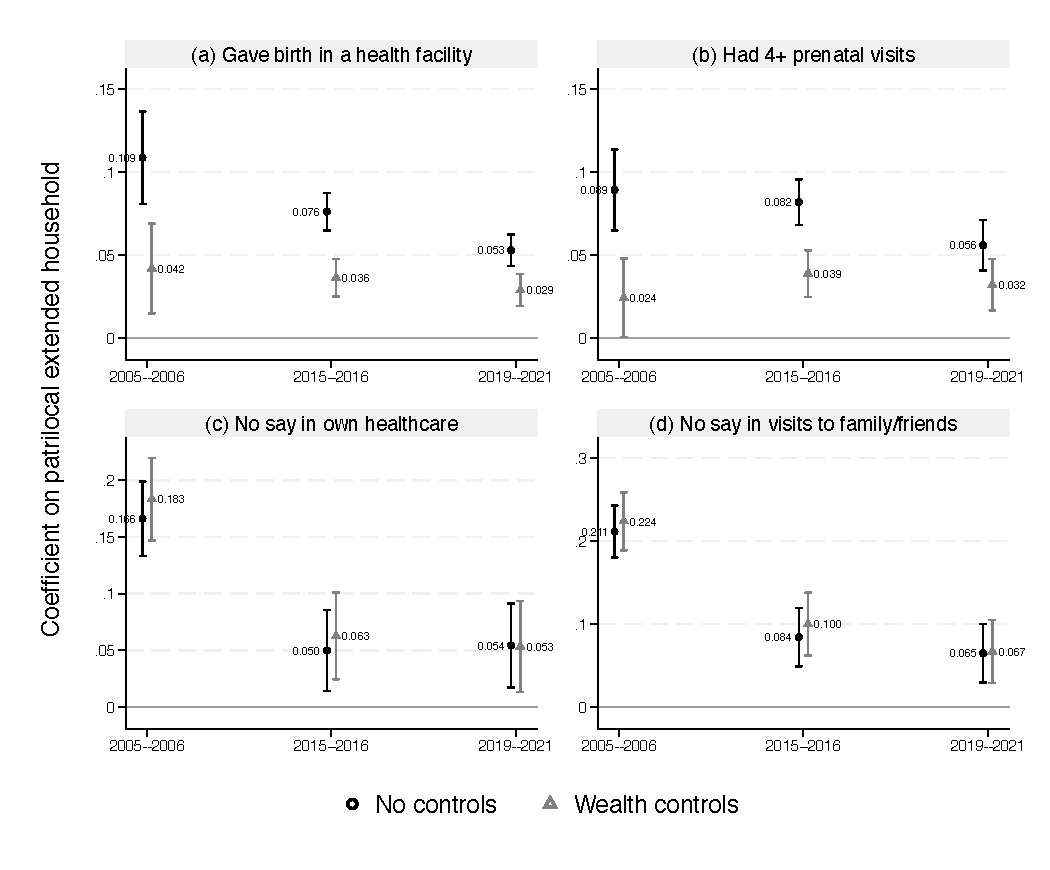
\includegraphics[width=\textwidth]{figures/figure1_patrilocaldiffs_wealthcontrols.pdf}
\end{center}

\vspace{1ex}
\small\scriptsize{\textsf{\textit{Note}: Data are from NFHS rounds 3 (2005--2006), 4 (2015--2016), and 5 (2019--2021).}}
\newline\small\scriptsize{\textsf{Points represent the coefficient $\beta_1$ on the patrilocal extended household indicator from the linear probability models shown in equations \ref{eq:nocontrols} and \ref{eq:controls}. Intervals represent 95\% confidence intervals on $\beta_1$.}}
\newline\small\scriptsize{\textsf{All four panels restrict the sample to ever-married women living in either nuclear or patrilocal extended household structures. Panels (a) and (b) use the recent birth sample, defined as ever-married women who gave birth 3--12 months before the survey.}}
\newline\small\scriptsize{\textsf{Panels (c) and (d) use the pregnant sample, defined as women who report being three or more months pregnant at the time of the survey and who were asked the decision-making questions ``Who usually makes decisions about healthcare for yourself?'' and ``Who usually makes decisions about visits to your family or relatives?''}}
\newline\small\scriptsize{\textsf{The outcomes ``No say in own healthcare'' and ``No say in visits to family/friends'' are constructed from these decision-making questions. Sample sizes for each regression match the number of women in the relevant subsample described in Table \ref{tab:sumstats}.}}

\end{flushleft}
\end{figure}


\subsection*{Patrilocal–nuclear differences decrease over time}

Table \ref{tab:narrowinggaps} presents estimates of changes in the gaps in outcomes between patrilocal extended and nuclear households over time.  Differences in women’s autonomy narrow substantially across survey rounds: between 2005–2006 and 2015–2016, the gap in having no say in healthcare decisions declines by 13.3 percentage points, while the gap in having no say in visiting family and friends declines by 13.6 percentage points. Over the full period from 2005 to 2021, the autonomy gaps decline by 13.7 and 17.3 percentage points, respectively.

In contrast, changes in gaps between women in patrilocal extended and nuclear households for maternal healthcare use outcomes are smaller. For institutional delivery, the gap declines by 3.9 percentage points over the full period. For prenatal care, the gap declines by 3.2 percentage points over the full period. Overall, convergence in maternal healthcare use across household structures is present, but more limited than for autonomy. 

Appendix Table D-1 shows that changes in household structure composition explain little of the improvement in autonomy and maternal health outcomes, with most gains driven by within-household-type changes. 

\begin{table}[H]
\sffamily
\caption{: The gap between patrilocal extended and nuclear households in women's autonomy and healthcare use is narrowing over time}
\label{tab:narrowinggaps}
\vspace{-4pt}

\begin{scriptsize}
\setlength{\tabcolsep}{6pt}
\renewcommand{\arraystretch}{1.6}

\makebox[\linewidth][c]{%
\begin{tabular}{lcccc}
\toprule
 & \multicolumn{1}{c}{\shortstack{$\delta$ (Eq.~\ref{eq:tworounds})\\2005--2006 vs.\\2015--2016}} & \multicolumn{1}{c}{\shortstack{$\delta$ (Eq.~\ref{eq:tworounds})\\2015--2016 vs.\\2019--2021}} & \multicolumn{1}{c}{\shortstack{$\delta_4$ (Eq.~\ref{eq:stacked})\\2005--2006 vs.\\2015--2016}} & \multicolumn{1}{c}{\shortstack{$\delta_5$ (Eq.~\ref{eq:stacked})\\2005--2006 vs.\\2019--2021}} \\\\
\midrule
No say in own healthcare$^1$&-0.106***&0.001&-0.107***&-0.135***\\
&(0.027)&(0.027)&(0.026)&(0.026)\\
&N = 8,158&N = 6,803&N = 11,127&N = 11,127\\
&&&&\\
No say in visits to family/friends$^1$&-0.117***&-0.025&-0.116***&-0.173***\\
&(0.026)&(0.027)&(0.026)&(0.025)\\
&N = 8,158&N = 6,803&N = 11,127&N = 11,127\\
&&&&\\
Gave birth in a health facility$^2$&-0.015&-0.023***&-0.014&-0.036**\\
&(0.015)&(0.007)&(0.015)&(0.015)\\
&N = 42,596&N = 67,666&N = 74,629&N = 74,629\\
&&&&\\
Had 4+ prenatal visits$^2$&0.005&-0.026**&0.002&-0.023\\
&(0.014)&(0.011)&(0.015)&(0.015)\\
&N = 42,596&N = 67,666&N = 74,629&N = 74,629\\
\bottomrule
\end{tabular}
%
}

\end{scriptsize}

\vspace{1ex}
\small\scriptsize{\textsf{\textit{Note}: Data are from NFHS rounds 3 (2005--2006), 4 (2015--2016), and 5 (2019--2021).}}
\newline
\small\scriptsize{\textsf{All samples are restricted to women living in either nuclear or patrilocal household structures.}}
\newline
\small\scriptsize{\textsf{$^1$ Uses the sample of ever-married women who report being three or more months pregnant at the time of the survey, and who were asked the questions `Who usually makes decisions about healthcare for yourself?'' and `Who usually makes decisions about visits to your family or relatives?''}}
\newline
\small\scriptsize{\textsf{$^2$ Uses the sample of ever-married women who report having given birth 3--12 months before the survey.}}
\end{table}

\section*{Discussion}

We use the most recent three waves of NFHS data to document an increase in the proportion of pregnant women in India who co-reside with their in-laws. Our results are surprising in the context of an influential prior literature that associates modernization with a shift toward nuclear households.  They are consistent with \cite{pesando2018global}, who find that in more recent data, there is no association between a country's level of human development and the share of women living in nuclear households.

The prior literature on family in India finds that extended families are less egalitarian than nuclear families; indeed, newly married women in patrilocal households occupy subordinate positions relative to their in-laws and their husbands' older brothers and their wives. Senior family members often dictate the details of the daily lives of co-resident daughters-in-law. Our findings are consistent with these long-standing descriptions of gender and age hierarchies.  We find that pregnant women in extended families have less say in their own healthcare and visits to family and friends than pregnant women in nuclear households, even controlling for wealth differences across these households. But over this period autonomy has also improved illustrating people's ideas are often shaped by multiple cultures \citep{allendorf2013schemas}.  Yet, pregnant women in extended families are more likely to use prenatal care and give birth in a health facility.  Differences in household level wealth explain much of the gap in healthcare use. 

Our results should be interpreted in the context of broad improvements in the availability of healthcare and of changes in the underlying determinants of women's status.  The time window we study begins in 2005, when the central government launched the National Rural Health Mission to expand contraceptive, prenatal, birth, and postnatal services.  As an illustration of these programs' reach, between 2005 and 2021, the proportion of women who gave birth in health facilities increased from about 40\% to about 90\% \citep{IIPS2007NFHS3,IIPS2021NFHS5}.  \cite{char2010influence} posit that these programs not only shaped access to reproductive healthcare, but also reduced the influence of mothers-in-law over the child-bearing patterns of their sons and daughters-in-law.  

Over the same period, the median pregnant woman's years of schooling increased from three years to nine years, and the average gap between her education and her husband's decreased from 2.1 years in 2005--2006 to 0.6 years in 2019--2021.  Such changes would matter for women's status.  This is not to say, however, that education necessarily increases a woman's autonomy within the home.  For example, \cite{srivastava2020time} compares women who are more or less educated than their co-resident mothers-in-law and finds that more educated women do not do less housework.  Households also got richer during this period in ways that shaped women's work: in 2005, about 17\% of extended households in which a pregnant woman resided primarily used liquefied petroleum gas (LPG) gas  for cooking, compared to 48\% in 2021.  The consequences of increasing patrilocal extended family residence would almost certainly have been different in the absence of these important society-level changes.

This study has a few limitations. Our measures capture use, but not the quality, of maternal healthcare. Four or more prenatal visits do not guarantee adequate, continuous, or comprehensive care. Similarly, the quality of institutional delivery varies across facilities.  In some settings, home birth is associated with lower neonatal mortality than private hospital birth \citep{coffey2025excess}. Further, our measures of autonomy rely on self-reported decision-making authority. They may not capture informal influence or everyday negotiations within the household. 

The NFHS data are cross-sectional and capture household structure only at the time of the survey. However, residence arrangements around marriage and childbirth can be fluid. Women may move between households frequently during pregnancy and postpartum. This movement could lead to error in our measurement of household structure.  Appendix Figure C-2 presents evidence that our finding of increasing extended family residence is unlikely to be caused by changes in visits to natal families during pregnancy.  It shows the type of household in which married men whose wives are currently pregnant live.  There is an 11 percentage point increase in the proportion who report being usual residents of patrilocal extended households between 2005 and 2021.

Although it is beyond the scope of this paper to investigate the reasons for pregnant women's increasing residence in patrilocal extended families, we note that fertility decline is likely an important factor.  Appendix Table A-1 shows the results of a Kitagawa decomposition that finds that about half of the increase in patrilocal family residence among pregnant women can be explained by the fact that in 2021, pregnant women had fewer prior live births than pregnant women did in 2005.  

Lower parity women are more likely to live with their in-laws than higher parity women in both time periods.  Women often move into their husband's parental houses soon after marriage \citep{breton2021modernisation} and are expected to begin childbearing soon after cohabitation begins \citep{ibarra2020desire}. Couples may separate from the extended household as they age and progress in parity. This is especially true if a new daughter-in-law joins the household.  

Another way in which declining fertility may cause increasing patrilocal residence among pregnant women has to do with lower fertility in their in-laws' generation.  If in-laws expect to be cared for by at least one son, and their sons have few or no brothers, the couple will face more pressure to continue living in an extended household.  Future research may seek to disentangle the extent to which increasing patrilocal extended family residence can be explained by lower parity progression among pregnant women, by lower fertility among their mothers-in-law, and by lower mortality among parents-in-law. 

This research also suggests that future research investigate how relationships within households are changing. Does being more ``needed'' by their in-laws give young women more autonomy?  How does the greater availability of healthcare and the increasing resources with which to pay for it change the experiences of pregnancy and birth?  How can we explain the greater use of healthcare among women in extended households relative to nuclear families of the same wealth?  Could in-laws be providing logistical or moral support to use healthcare that makes a difference?  Perhaps in-laws are willing to spend resources on the care of their daughters-in-law that couples are not.  Understanding how economic resources and family relationships shape women's lives remains important for understanding women's well-being. 





\subsection*{Disclosure about use of AI}

ChatGPT was used as a coding assistant. Researchers prompted ChatGPT to follow specified pseudocode and previously written code produced by the researchers without AI assistance. ChatGPT was used to generate draft Stata and LaTeX code for reproducing, formatting, and displaying tables and figures. All AI-assisted code was manually reviewed, verified, and adjusted by the researchers before being used in the analysis or manuscript.




% TIPS: 
% 	- Use an en-dash (--) for all minuses, page spans, years, etc.  
%	- Use, e.g., \cite{ }, \citep{ }, and \citeauthor{ } for in-text citations (ensure that no extra brackets are created). 
%	- Use \% for\% symbol (unless there is a real reason for spelling it out)
%	- Italics should not be used to emphasize portions of text.
%		- See the "Cheat Sheet" for further information.


%%%%%%%%%%%%%%%%%%%%%%%%% IN-TEXT TABLES & FIGURES %%%%%%%%%%%%%%%%%%%%%%%%%

% NOTE! All tables and figures must be first mentioned in the text, then the imagery follows (after the full stop): 
% - Please use \floatbarrier or [H] to ensure that all tables and figures come AFTER a paragraph is completed (i.e., not within the paragraph). 


% - Please ensure to format all tables, figures, graphs, etc. with the appropriate caption headings and sizing. 
%     - See the LaTeX formatting cheat sheet (points 2–3). 
%     - If you have more than ten figures/tables, PLEASE INSERT \hspace{} (e.g., \hspace{-1em}) before the caption.

% --------------------------------- TABLE TEMPLATE ---------------------------------

%		\begin{table}[H]
%		\sansmath
%		\sffamily
%		\captionsetup{style=CAPFIG}
%		\caption{\label{tab:estimated-parameters}Estimated parameters and standard errors}\vspace{-4pt}
%		\begin{scriptsize}
%		\setlength{\tabcolsep}{4pt}
%  	 \begin{tabular}{ldddD{.}{.}{2.5}}                        %%%% CHANGE according to your table.
%		\hline
%		\\[-3pt]
%		{ }& \multicolumn{1}{c}{\textbf{XXX}} &   & \multicolumn{1}{c}{\textbf{XXX}} &  \\            %%%% DELETE if you do not require two lines for headings.
%		\multicolumn{1}{c}{\textbf{XXXX}} & \multicolumn{1}{c}{\textbf{XXXX}} & \multicolumn{1}{c}{\textbf{XXXX}} & 		\multicolumn{1}{c}{\textbf{XXXX}} & \multicolumn{1}{c}{\textbf{XXXX}}\\
%		\\[2pt]
%		\hline
%		\\[-3pt]
% 	Cell & Cell & Cell & Cell & Cell\\[2pt]
% 	Cell & Cell & Cell & Cell & Cell\\[2pt]
% 	Cell & Cell & Cell & Cell & Cell\\[2pt]
% 	Cell & Cell & Cell & Cell & Cell\\[2pt]
% 	Cell & Cell & Cell & Cell & Cell\\[2pt]
% 	Cell & Cell & Cell & Cell & Cell\\[2pt]
% 	Cell & Cell & Cell & Cell & Cell\\[2pt]
% 	Cell & Cell & Cell & Cell & Cell\\[2pt]
% 	Cell & Cell & Cell & Cell & Cell\\
%		\\[3pt]
%		\hline
%		\end{tabular}
%		\end{scriptsize}
%		To place a NOTE, following the table:
%  	 \vspace{1ex} % if at least one note
%		\small\scriptsize{\textsf{\textit{Source}: Total fertility rate (1949--2002) comes from \citet{Lu:2009} ``Sixty Years of New China Population.'' Sex ratio at birth (1960--1988) comes from \citet{Liang:1993}. Sex ratio at birth (1989--2000) comes from the China Population Statistics Yearbook.}}
%		% notes terminate in full stop, newline only for new note type -- not per sentence
%\end{table}


% --------------------------------- FIGURE TEMPLATE ---------------------------------

%		\begin{figure}[H]
%		\begin{flushleft}\captionsetup{style=CAPFIG} % leave CAPFIG
%		\caption{!!Caption} 
%		\label{!!Label}
%		\vspace{0em} % vspace, adjust if necessary, can be negative
%		\includegraphics[width=0.8\textwidth]{!!PathToGraphic} % width and alignment (here \center) can be changed
%		To place a NOTE, following the figure
%   \vspace{1ex} % if at least one note
%		\small\scriptsize{\textsf{\textit{Source}: Total fertility rate (1949--2002) comes from \citet{Lu:2009} ``Sixty Years of New China Population.'' Sex ratio at birth (1960--1988) comes from \citet{Liang:1993}. Sex ratio at birth (1989--2000) comes from the China Population Statistics Yearbook.}}
%		\end{flushleft}
%		\end{figure}
%		\FloatBarrier (if necessary)

% --------------------------------- EQUATION TEMPLATE --------------------------------- 

%	\vspace{-6pt}
%	\begin{equation}
%	\beta^{-1}\log(c)h({c\kappa}) < e(a;1) - e(a;c) < {\beta ^{ - 1}}\log(c)h(\kappa)
% 			- If equation is too big, use	\small or \normalsize
%	\end{equation}
%	\vspace{-6pt}

% TIP: Use periods and commas at the end of the equation.

% --------------------------------- HYPOTHESIS TEMPLATE ---------------------------------

%	\vspace{10pt}
%	\parbox{11.75}{\textit{Hypothesis 1:} Text}
%	\vspace{10pt}

% For more mathematical functions, see the cheat sheet. 

%%%%%%%%%%%%%%%%%%%%%%%%% REFERENCES %%%%%%%%%%%%%%%%%%%%%%%%%

\section*{Conflict of Interest}
The authors have no conflicts of interest to disclose.

\newpage
\addcontentsline{toc}{section}{\numberline{}References}
\bibliographystyle{DemRes}
\bibliography{references} % bibliography file
\nocite{*}


\end{document}


